\section{Versuchsaufbau}
\label{sec:Versuchaufbau}
Der bei diesem Versuch verwendete Aufbau ist in Abbildung $\ref{fig:Aufbau}$ dargestellt.

\begin{figure}[H]
  \centering
  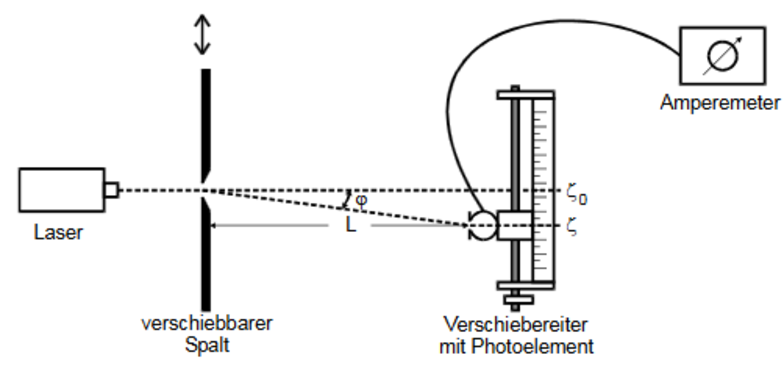
\includegraphics{ressources/Aufbau.pdf}
  \caption{Versuchsaufbau, \cite{skript}.}
  \label{fig:Aufbau}
\end{figure}

Mit einem He-Ne-Laser wird ein Einzelspalt und im späteren Teil des Versuchs auch ein Doppelspalt beleuchtet. Dabei ist zu beachten, das wie zuvor erwähnt die Breite des Spalts kleiner sein muss als die Wellenlänge des He-Ne-Laser von $\lambda = \SI{633}{\nano\meter}$.
Der Abstand zwischen der Beugungsebene und der Beobachtungsebene beträgt $\SI{100}{\centi\meter}$ - $\SI{120}{\centi\meter}$. In der Beugungsebene ist ein verschiebbarer Detektor installiert, der die Intensität des einfallenden Lichtes registriert. Diese sogenannte Photodiode gibt einen kleinen Strom ab der mit einem Amperemeter gemessen wird.
